\section{Git}

\begin{figure}[ht]
  \begin{center}
  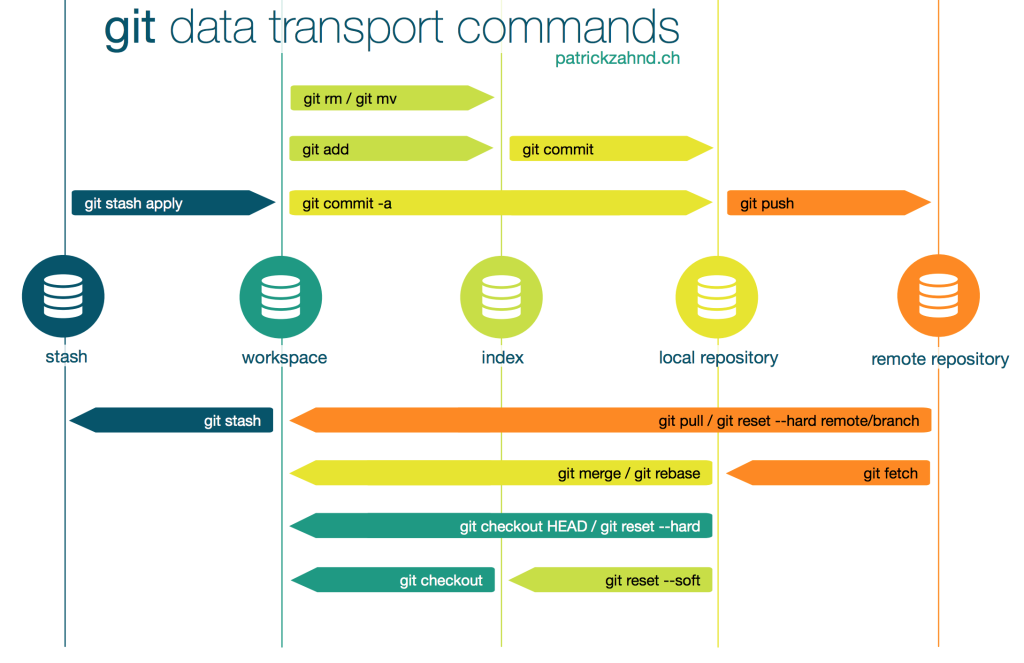
\includegraphics[keepaspectratio,width=0.9\textwidth]{Pictures/git-cheatsheet1.png}
  \caption{Git CheetSheet from
    \url{https://www.quora.com/What-is-the-best-Git-cheat-sheet}}
  \label{fig:HardwareStructure}
  \end{center}
\end{figure}

\subsection{Setting up a repository}

\begin{verbatim}
git init --bare /path/to/bare/repo.git
git clone /path/to/bare/repo.git /path/to/work
echo 123 > afile.txt
git add .
git config --local user.name adelphus
git config --local user.email adelphus@example.com
git commit -m "added afile"
git push origin master
\end{verbatim}

\subsection{Cleansing and Space Savings}

\begin{verbatim}
  git clean -d -f -i # interactive cleaning 
  git prune --progress  # delete objects w/o references
  git gc --auto
  git gc --aggressive  
  git remote prune origin # delete remotely removed branches 
\end{verbatim}

A more complete way is to abandon all commit histories and just start over fresh:
\begin{verbatim}
  rm -rf .git
  git init
  git add .
  git commit -m "Initial commit"
  -- push to the github remote repos ensuring you overwrite history
  git remote add origin git@github.com:<YOUR ACCOUNT>/<YOUR REPOS>.git
  git push -u --force origin master
\end{verbatim}

